\documentclass[11pt,a4paper]{article}

\usepackage{classeRapport}
\usepackage{tikz,pgfplots}
\usetikzlibrary{positioning}
\usetikzlibrary[topaths]
\usepackage{algorithmeUTF8}
\usepackage{pgfplots}
\pgfplotsset{compat=1.15}
\usepackage{mathrsfs}
\usetikzlibrary{arrows}
\setlength{\headheight}{13.59999pt}

\newcount\mycount

\definecolor{qqwuqq}{rgb}{0,0,0}
\definecolor{sudaqq}{rgb}{0,0,0}

\begin{document}

\PageDeGarde	
{unknown.png} % image sur la page de garde
{Recherche opérationel - TP} % titre principal
{Balade en ville} % sous-titre
{Alexis \textsc{Imbert}\\
 Brice \textsc{Grindel}} % nom
{RO - ITI - 2022-2023} % bas de page

\Page{INSALogo}{unknown.png} % logo de bas de page (en bas a droite)

 
\tableofcontents
\newpage
\section{Etape 1 : Modéliser, définir le problème formel, associer une classe de complexité}
\begin{itemize}
    \item 
    \begin{itemize}
        \item On propose de représenter par le graphe 
        \begin{itemize}
            \item Les noeuds représenteront les intersections, les addresses et les arrêts de métros.
            \item Les arrêtes représenteront les portions de route ou entre 2 stations de métros.
        \end{itemize}
        Si le métro est proche de d'un intersection on peut faire l'approximation que c'est le même noeud.

        Représentation sagitale :

        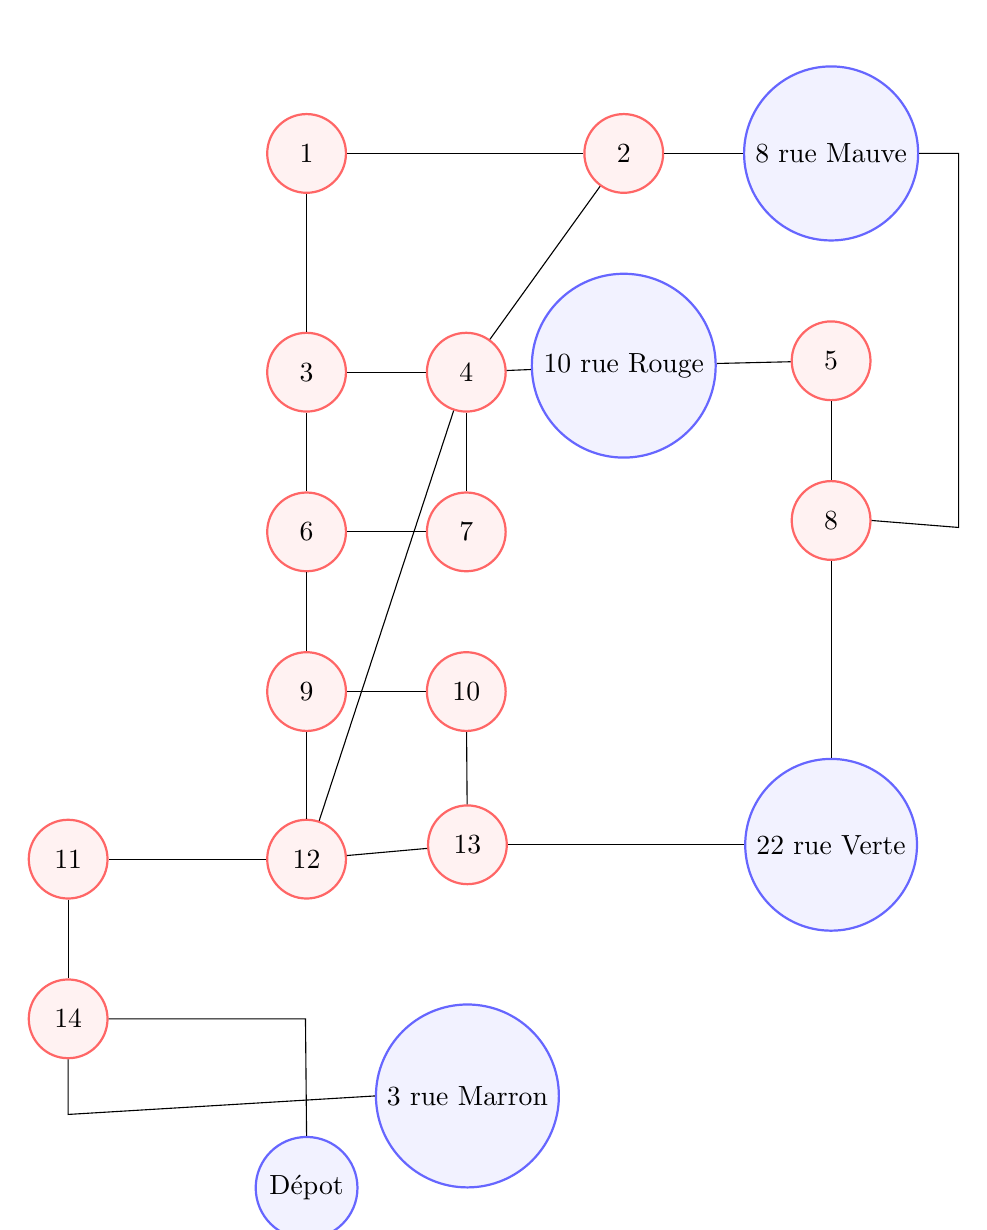
\begin{tikzpicture}[
    scale=0.5,
    roundnode/.style={circle, draw=red!60, fill=red!5, thick, minimum size=10mm},
    addresse/.style={circle, draw=blue!60, fill=blue!5, thick, minimum size=10mm},
]
    %node
    \node[roundnode] (1) {1};
    \node[roundnode] (9) [right=3 of 1] {2};
    \node[addresse] (10) [right=of 9] {8 rue Mauve};
    \node[addresse] (14) [below=of 9] {10 rue Rouge};
    \node[roundnode] (11) [below=of 10] {5};
    \node[roundnode] (12) [below=of 11] {8};
    \node[addresse] (13) [below=2.5 of 12] {22 rue Verte};
    \node[roundnode] (2) [below=1.75 of 1] {3};
    \node[roundnode] (3) [below=of 2] {6};
    \node[roundnode] (16)[right=of 3] {7};
    \node[roundnode] (15)[right=of 2, left=of 14,above=of 16] {4};
    \node[roundnode] (4) [below=of 3] {9};
    \node[roundnode] (5) [below=1.1 of 4] {12};
    \node[roundnode] (17)[below=of 16, right=of 4] {10};
    \node[roundnode] (18)[below=of 17, right=of 5,left=3 of 13] {13};
    \node[roundnode] (7) [left=2 of 5] {11};
    \node[roundnode] (8) [below=of 7] {14};
    \node[addresse] (6) [below=1.5 of 18] {3 rue Marron};
    \node[addresse] (depot) [below left=of 6,below=3 of 5] {Dépot};
    
    %lines
    \draw (1) -- (9);
    \draw (1) -- (2);
    \draw (2) -- (3);
    \draw (3) -- (4);
    \draw (3) -- (16);
    \draw (15) -- (16);
    \draw (4) -- (5);
    \draw (4) -- (17);
    \draw (5) -- (7);
    \draw (5) -- (18);
    \draw (17) -- (18);
    \draw (12) -- (13);
    \draw (12) -- (11);
    \draw (14) -- (11);
    \draw (14) -- (15);
    \draw (2) -- (15);
    \draw (18) -- (13);
    \draw (7) -- (8);
    \draw (9) -- (10);
    \draw (5) -- (15) -- (9);
    \draw (10.east) -- ++(1,0) -- ++(0,-9.5) -- (12.east);
    \draw (8.east) -- ++(5,0) -- (depot.north);
    \draw (8.south) -- ++(0,-1.4) -- (6.west);
\end{tikzpicture}

        Pour simplifier le graphe : on peut extraire un graphe de distance géodésique entre les adresses tel que : 
        \begin{itemize}
            \item Les noeuds représenteront les addresses
            \item Les arrêtes représenteront les chemins reliant ces addresses.
        \end{itemize}
        Représentation sagitale :
        \begin{center}
    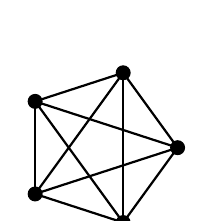
\begin{tikzpicture}[line cap=round,line join=round,>=triangle 45,x=1cm,y=1cm]
        \draw [line width=0.8pt,color=sudaqq] (0.30901699437494745,0.9510565162951535)-- (0.30901699437494745,0.9510565162951535);
        \draw [line width=0.8pt,color=sudaqq] (-0.8090169943749473,0.5877852522924732)-- (0.30901699437494745,0.9510565162951535);
        \draw [line width=0.8pt,color=sudaqq] (-0.8090169943749475,-0.587785252292473)-- (0.30901699437494745,0.9510565162951535);
        \draw [line width=0.8pt,color=sudaqq] (0.30901699437494723,-0.9510565162951536)-- (0.30901699437494745,0.9510565162951535);
        \draw [line width=0.8pt,color=sudaqq] (1,0)-- (0.30901699437494745,0.9510565162951535);
        \draw [line width=0.8pt,color=sudaqq] (-0.8090169943749473,0.5877852522924732)-- (-0.8090169943749473,0.5877852522924732);
        \draw [line width=0.8pt,color=sudaqq] (-0.8090169943749475,-0.587785252292473)-- (-0.8090169943749473,0.5877852522924732);
        \draw [line width=0.8pt,color=sudaqq] (0.30901699437494723,-0.9510565162951536)-- (-0.8090169943749473,0.5877852522924732);
        \draw [line width=0.8pt,color=sudaqq] (1,0)-- (-0.8090169943749473,0.5877852522924732);
        \draw [line width=0.8pt,color=sudaqq] (-0.8090169943749475,-0.587785252292473)-- (-0.8090169943749475,-0.587785252292473);
        \draw [line width=0.8pt,color=sudaqq] (0.30901699437494723,-0.9510565162951536)-- (-0.8090169943749475,-0.587785252292473);
        \draw [line width=0.8pt,color=sudaqq] (1,0)-- (-0.8090169943749475,-0.587785252292473);
        \draw [line width=0.8pt,color=sudaqq] (0.30901699437494723,-0.9510565162951536)-- (0.30901699437494723,-0.9510565162951536);
        \draw [line width=0.8pt,color=sudaqq] (1,0)-- (0.30901699437494723,-0.9510565162951536);
        \draw [line width=0.8pt,color=sudaqq] (1,0)-- (1,0);
        \begin{scriptsize}
            \draw [fill=sudaqq] (0.30901699437494745,0.9510565162951535) circle (2.5pt);
            \draw [fill=sudaqq] (-0.8090169943749473,0.5877852522924732) circle (2.5pt);
            \draw [fill=sudaqq] (-0.8090169943749475,-0.587785252292473) circle (2.5pt);
            \draw [fill=sudaqq] (0.30901699437494723,-0.9510565162951536) circle (2.5pt);
            \draw [fill=sudaqq] (1,0) circle (2.5pt);
        \end{scriptsize}
    \end{tikzpicture}
\end{center}
    \end{itemize}
        

        \item Le graphe est non orienté. Pour le passage d'addresse en paramètre on peut passer les arrêtes sur lesquels sont ces arrêtes.

        
    \item On a deux problèmes formel sous jacents.
    \begin{itemize}
        \item La recherche de plus cours chemin
        \item La recherche d'un cycle hamiltonien
    \end{itemize}
    Ce problème peut se ramener au problème du voyageur de commerce.
    \item Le problème du voyageur de commerce fait parti des problèmes NP-complet. C'est à dire que la résolution de ce type de problème est exponentiel.
    Toutefois nous ne sommes pas obliger d'abandonner tout de suite car ici le graphe est assez petit : seulement 5 addresses à parcourir.

    Le problème de plus court chemin peut etre résolu par l'algorithme de Dijkstra qui a une résolution polynomiale. Dans notre cas comme la valuation de toutes les arrêtes est égale à 1, cela revient à un parcours en largeur.
\end{itemize}
\section{Etape 2 : l'algoritme}
\paragraph{Etat de l'art}
\url{https://www.datavis.fr/playing/salesman-problem}

Une première solution est le brut force : énumération de tout les chemins possible et choix du plus cours. 
\paragraph{Algorithme}

\section{Etape 3 : L'implémentation}
% mettre le code dans le rapport ?
\section{Etape 4 : L'adaptation}
\begin{itemize}
    \item Dans notre modélisation on peut isoler les arrêtes du métro à part et vérifier si le chemin emprunté lors de la création du graphe simplifié passe par l'une des arrêtes du métro. 
    Dans ce cas on peut affecter une variable booléenne.
    \item Si le métros tombe en panne il n'y aucun changement dans l'algorithme : on a juste à rentré un nouveau fichier .txt sans les arrêtes liée au métro
    \item Pour afficher les 2 résultats : on fait tourner l'algorithme sur les 2 fichiers d'entrée : avec et sans le métro.
\end{itemize}

\end{document}
